% titlepage-demo.tex
\documentclass{beamer}
\usetheme{Boadilla}
\usepackage{multirow}
\usepackage[absolute,overlay]{textpos} 
\newenvironment{reference}[2]{% 
  \begin{textblock*}{\textwidth}(#1,#2) 
      \footnotesize\it\bgroup\color{red!50!black}}{\egroup\end{textblock*}} 



\begin{document}
	

\begin{frame}[t]{Summary}
	
	\begin{enumerate}
		\item \small{Segment-based Representation (SB)}
		\begin{itemize}
			\item \small{Investigate different strategies to \\
				decompose a video into segments; \\
				study the optimal segment length.}
			%\item Outcome: PCM 2012, \textbf{JSPS \\2014} (journal).
			\item \textit{Challenges: uncontrolled capturing, 
				\\large content variation.}
		\end{itemize}
		\item Sum-Max Video Aggregation (SM)
		\begin{itemize}
			\item An efficient method to aggregate\\
			local features into video feature \\
			representation.
			%\item Outcome: ICIP 2014.
			\item \textit{Challenges: uncontrolled capturing,
				\\ large scale dataset.}
		\end{itemize}
		\item Event-driven Multiple Instance \\
		Learning (EDMIL)
		\begin{itemize}
			\item A method to leverage the event\\
			description to learn key evidences \\
			for complex event detection.
			%\item Outcome: ACM MM 2015.
			\item \textit{Challenges: uncontrolled capturing, 
				\\large content variation.}
		\end{itemize}
	\end{enumerate}
	
	\begin{tikzpicture}[remember picture,overlay]  
	\node [xshift=-3cm,yshift=-4.5cm] at (current page.north east)
	{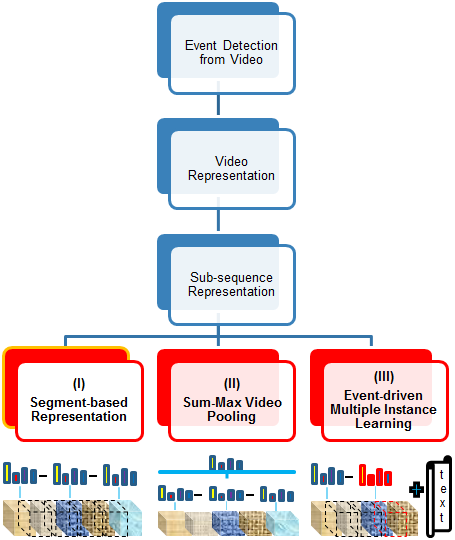
\includegraphics[width=5cm,height=7.5cm]{images/part1/contribution2.png}};
	\end{tikzpicture}
	
\end{frame}


\begin{frame}[t]{Summary (cont'd)}
	
	
	\bigskip
	
	\begin{columns}
		\begin{column}{0.5\textwidth}
			\centerline{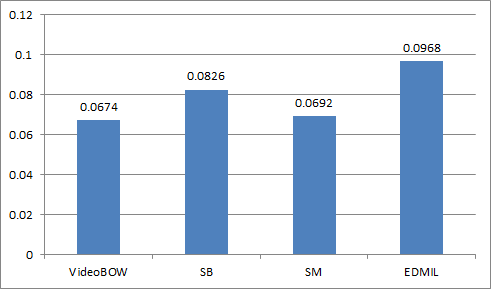
\includegraphics[width=1\textwidth]{images/summary3.png}}
			\small{Our methods (SB, SM and EDMIL) improve the baseline VideoBOW by \textbf{23\%}, \textbf{3\%} and \textbf{44\%} respectively on the large scale MED 2011 dataset.}
		\end{column}
		
		\begin{column}{0.5\textwidth}
			\centerline{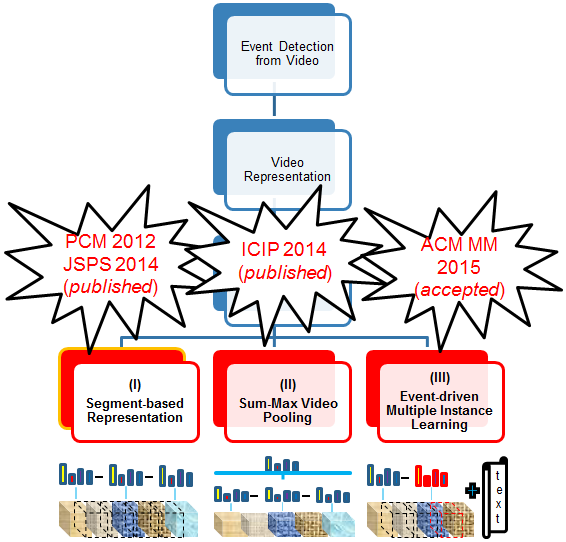
\includegraphics[width=1\textwidth]{images/summary2.png}}
			\small{Achievements: PCM2012 \textit{(Rank C)}, ICIP2014 \textit{(Rank B)}, ACMMM2015 \textit{(Rank A)}; JSPS2014 \textit{(IF: 0.6)}.}
		\end{column}
	\end{columns}
	\bigskip
	
	
\end{frame}

\begin{frame}[c]{}
	
	\centering{Thank you for your attention!}
\end{frame}

\end{document}